\section{Background}

\subsection{Settings}

\subsubsection{Bandit Setting}

For simplicity, we first present the main results in the standard bandit setting, and then discuss several general settings.

In the standard bandit setting, we have $n = 1$. At each time step $t$, the agent takes an action $A_t \in [h]$ according to some strategies, and then it observes a reward $r_{A_t} \in \sR$. The agent then uses the reward to improve its action selection strategies. After such $T$ time steps, the performance of the agent's strategy is measured by the (expected) regret,
\begin{equation*}
    \ell \triangleq \r^{\max} \cdot T - \sE \left[ \sum\limits_{t=0}^{T-1}{  \rvr_{A_t}  } \right] = \sum\limits_{t=0}^{T-1}{ \sE \left[ \rvtilder_{A_t} \right] },
\end{equation*}
where the expectation is taken over the randomness of action selection, if the agent is using stochastic strategies.

\subsubsection{Episodic Markov decision process (MDP)}

The episodic MDP setting recovers the bandit setting as a special case. The environment randomly select a starting state $\rvs_i^0 \in \sR^d$. At each time step $t$, the agent takes one action $A_t \in [h]$ according to some strategies, and then it observes a reward $r_{A_t} \in \sR$ and next state $S_{t+1} \sim \sP\left( \cdot \middle| S_t, A_t \right)$. After such $H$ steps, the agent observes an ending state $S_H$, and the current trajectory terminates. At the next time step, the agent will observe a new starting state $\rvs_i^0$ provided by the environment. Since we use policy gradient method (no value learning), the agent updates its NN policy weights using the cumulative reward collected after each trajectory terminates.

\subsection{Neural Network (NN) Policy}


\subsection{Policy Gradient Method}

\begin{algorithm}[h]
   \caption{Policy Gradient Method Mixed with Uniform Exploration}
\label{alg:policy_gradient_uniform_exploration}
\begin{algorithmic}
   \STATE {\bfseries Input:} state feature vectors $\rvs_i$
   \STATE Initialize $\rvw_r \sim \gN\left( 0, \sigma \cdot \rmI \right)$, $\forall r \in [m]$, $\rva_k \sim \gN(0, \rmI)$, $\forall k \in [h]$.
   \FOR{$t=0$ {\bfseries to} $T-1$}
   \IF{$t < \sqrt{T}$}
   \STATE Uniformly randomly take action $A_{i,t}$. 
   \STATE Observe reward and next state.
   \ELSE
   \STATE Take action $A_{i,t} \sim \rvpi_{i}\left(\cdot \middle| S_{i,t} \right)$. 
   \ENDIF
   \STATE $\rvw_r(t+1) = \rvw_r(t) - \eta \cdot \frac{d\ell}{d \rvw_r(t)}$, $\forall r \in [m]$.
   \ENDFOR
\end{algorithmic}
\end{algorithm}

The objective of our analysis is the policy gradient method, mixed with uniform exploration, as shown in shown in \cref{alg:policy_gradient_uniform_exploration}. The reason why we need exploration will be explained later on, and technically it seems cannot be eliminated.

The policy gradient method works as follows. After initialization, the policy net $\rvpi$ will be updated using policy gradient calculated from collected reward. In the first $\sqrt{T}$ steps, actions are selected up to an uniform distribution over all actions. After that the NN policy $\rvpi$ is used to select actions.

\subsection{Main Results}
\label{subsec:main_results}

The first main result of the bandit setting is summarized in \cref{thm:main_result}.

\begin{thm}
\label{thm:main_result}
    Given a two layer NN policy $\rvpi$, with number of parameters $m \in \tilde{\Theta}\left( \frac{n^{10}}{c^4 \delta^4 \varepsilon^2} \right)$, $\eta \in \Theta\left( \frac{c^2 \delta^2}{16 n^4 h m \left( \log{\left(4m\right)} \right)^2} \right)$, the regret of \cref{alg:policy_gradient_uniform_exploration} satisfies $\sum\limits_{t=1}^{T}{ \rvpi_i\left( \rmW(t) \right)^\top \rvtilder_i } \le  \frac{8 n^4 \sqrt{h}}{c^2 \delta^2} \cdot \tilde{O}\left( \sqrt{T} \right)$.
\end{thm}
\begin{proof}
According to \cref{alg:policy_gradient_uniform_exploration}, the first $\sqrt{T}$ steps are played by uniformly taking actions, and they totally contribute $\sqrt{T}$ regret. After the first $\sqrt{T}$ steps, in expectation every arm is pulled $\frac{\sqrt{T}}{h}$ times, by \cref{thm:regret_convergence}, 
\begin{equation*}
\begin{split}
    \rvpi_i\left( \rmW(t) \right)^\top \rvtilder_i \le O\left( \frac{n^4}{\eta m c^2 \delta^2 \sqrt{T}} \right),
\end{split}
\end{equation*}
for $t = \sqrt{T}$. Denote $\varepsilon \triangleq \frac{n^4}{\eta m c^2 \delta^2 \sqrt{T}}$. By \cref{subsec:playing_phase}, $\rvpi_i\left( \rmW(t) \right)^\top \rvtilder_i \le \varepsilon$, $\forall t \ge \sqrt{T}$. Therefore the regret can be upper bounded by the sum of two parts,
\begin{equation*}
\begin{split}
    \sum\limits_{t=1}^{T}{ \rvpi_i\left( \rmW(t) \right)^\top \rvtilder_i } &\le \sqrt{T} \cdot 1 + \left(T - \sqrt{T} \right) \cdot \varepsilon \\
    &\le \frac{8 n^4 \sqrt{h}}{c^2 \delta^2} \cdot \log{\left(4m\right)} \cdot \sqrt{T} \\
    &\le \frac{8 n^4 \sqrt{h}}{c^2 \delta^2} \cdot \tilde{O}\left(\sqrt{T}\right). \qedhere
\end{split}
\end{equation*}
\end{proof}

\section{Theoretical Analysis}

We present more detailed analysis than \cref{subsec:main_results}. We first show the bandit case. Note that in the proof of \cref{thm:regret_convergence}, the $T$ steps are divided into two parts. In the first $\sqrt{T}$ exploration phase, we uniformly sample actions, and use collected rewards to make the expected regret of NN policy converge to smaller than $\varepsilon$. And in the second commit phase, we use NN policy to play, and because of the expected reward is small, we have the gradient norm lower bounded by positive constant times regret, so the NN policy will keep improving itself. Therefore our analysis will also be partitioned into two parts.

\subsection{Exploring Phase}
\label{subsec:exploring_phase}

In the exploring phase, we uniformly sample actions and rewards to update NN policy. The convergence of policy regret mainly relies on the following ``smoothness" like property over NN weights.

\begin{lem}
\label{lem:smoothness}
    Given weights $\rmW \triangleq \left[ \rvw_1, \rvw_2, \dots, \rvw_m \right]$, and $\rmW^\prime \triangleq \left[ \rvw_1^\prime, \rvw_2^\prime, \dots, \rvw_m^\prime \right]$. Denote $\rvpi_i\left( \rmW \right)$ and $\rvpi_i\left( \rmW^\prime \right)$ as the neural network policies parameterized by $\rmW$ and $\rmW^\prime$, respectively. $\forall i \in [n]$,
\begin{equation*}
\begin{split}
    &\rvpi_i\left( \rmW^\prime \right)^\top \rvtilder_i \le \rvpi_i\left( \rmW \right)^\top \rvtilder_i + \left\langle \frac{d \rvpi_i\left( \rmW \right)^\top \rvtilder_i }{d\left( \rmW \right)}, \rmW^\prime - \rmW \right\rangle \\
    &\qquad + 4 \sqrt{m \log{\left(4m\right)}} \cdot \rvpi_i\left( \rmW \right)^\top \rvtilder_i \cdot \left\| \rmW^\prime - \rmW \right\|_F \\
    &\qquad + 4 h m \log{\left(4m\right)} \cdot \left\| \rmW^\prime - \rmW \right\|_F^2.
\end{split}
\end{equation*}
\end{lem}

Combining this smoothness condition with other objective properties like convexity one can prove convergence results. However, the policy regret is non-convex function of weights. Therefore we need the recent results in overparameterized NN optimization, i.e., the gradient coupling and gradient (lower) bounds.

\begin{lem}
\label{lem:gradient_coupling}
	Define the pseudo gradient as,
\begin{equation*}
\begin{split}
	\frac{d \tilde{\ell}}{d \rvw_r(t)} &\triangleq \frac{1}{n} \cdot \sum\limits_{i=1}^{n}{ \sum\limits_{k=1}^{h}{ \tilde{r}_{i,k} \cdot \pi_{i,k}(t) \cdot \left( \sum\limits_{k^\prime = 1}^{h}{ a_{k^\prime,r}  \cdot v_{k^\prime,k,i}(t) } \right) } } \\
	&\qquad { { \cdot \sI\left\{ \rvw_r(0)^\top \rvs_i > 0 \right\} \cdot \rvs_i } },
\end{split}
\end{equation*}
where $v_{k^\prime,k,i}(t)$ is defined as,
\begin{equation*}
	v_{k^\prime,k,i}(t) = \begin{cases}
    1 - \pi_{i,k^\prime}(t), & \text{if $k^\prime = k$}, \\
    - \pi_{i,k^\prime}(t), & \text{otherwise}.
  \end{cases}
\end{equation*}
	For any $\tau > 0$, with probability at least $\frac{1}{2} \cdot \left( 1 - \frac{\sqrt{2}n\tau}{\sqrt{\pi}\sigma} \right)$, $\forall t \in O\left(\frac{\tau}{\eta  \sqrt{\log{m}}}\right)$, $\forall r \in [m]$,
\begin{equation}
	\frac{d\ell}{d \rvw_r(t)} = \frac{d \tilde{\ell}}{d \rvw_r(t)}.
\end{equation}
\end{lem}

The true gradient can be calculated as,
\begin{equation*}
\begin{split}
    \frac{d\ell}{d \rvw_r(t)} &= \frac{1}{n} \cdot \sum\limits_{i=1}^{n}{ \sum\limits_{k=1}^{h}{  \tilde{r}_{i,k} \cdot \pi_{i,k}(t) \cdot \left( \sum\limits_{k^\prime = 1}^{h}{ a_{k^\prime,r}  \cdot v_{k^\prime,k,i}(t) } \right) }} \\
    &\qquad  {{ \cdot \sI\left\{ \rvw_r(t)^\top \rvs_i > 0 \right\} \cdot \rvs_i } }.
\end{split}
\end{equation*}

\cref{lem:gradient_coupling} means $\sI\left\{ \rvw_r(t)^\top \rvs_i > 0 \right\} = \sI\left\{ \rvw_r(0)^\top \rvs_i > 0 \right\} $ for bounded time steps $t$ with constant probability, therefore the true gradient can be replaced with the simpler pseudo gradient.

The next lemma shows that the true gradient norm is upper bounded by regret, which is quite standard.

\begin{lem}
\label{lem:gradient_upper_bound}
With probability at least $\frac{1}{2}$,
\begin{equation*}
\begin{split}
	\left\| \frac{d\ell}{d \rvw_r(t)} \right\|_2 \le \frac{2 \sqrt{\log{\left(4m\right)}}}{n} \cdot \sum\limits_{i=1}^{n}{ \rvpi_{i}(t)^\top \rvtilder_i }.
\end{split}
\end{equation*}
\end{lem}

Now comes the key part of the recent progresses of overparameterized NN optimization theory, with constants probability, the pseudo gradient norm is lower bounded by the loss. However, due to the inherent difference of RL and supervised learning, our result contains an exploration item, which lead to the necessity of the exploration phase in \cref{alg:policy_gradient_uniform_exploration}. 

\begin{lem}
\label{lem:gradient_lower_bound}
	Denote $i^*(t) \triangleq \argmax\limits_{i \in [n]}\left\{\rvpi_i(t)^\top \rvtilder_i \right\}$, $k^*(t) \triangleq \argmax\limits_{k \in [h]}\left\{ r_{i^*(t),k} \right\} = \r_{i^*(t)}^{\max}$, i.e., the optimal arm of state $i^*(t)$. If $\pi_{i^*(t), k^*(t)}(t) > c > 0$, where $c$ is an exploration constant, then with probability $\Omega\left( \frac{\delta}{n} \right)$,
\begin{equation*}
\begin{split}
	\left\| \frac{d\tilde{\ell}}{d \rvw_r(t)} \right\|_2 \ge \Omega\left( \frac{c\delta}{n^2} \right) \cdot \rvpi_{i^*(t)}(t)^\top \rvtilder_{i^*(t)} .
\end{split}
\end{equation*}
\end{lem}

\cref{lem:gradient_lower_bound} is a generalization of recent overparameterized NN optimization results into the RL field. With this result, once the policy regret is large, with enough exploration of the optimal action (the constant $c$ here), the pseudo gradient norm will also be large (with constant probability). Therefore, combining \cref{lem:gradient_lower_bound} with \cref{lem:gradient_coupling}, we can get the true gradient norm is also large, which is necessary for objective progress and regret convergence. Using all the lemmas presented in this section, we get the convergence result for the exploring phase.

\begin{thm}
\label{thm:regret_convergence}
    Assume $m \in \tilde{\Theta}\left( \frac{n^{10}}{c^4 \delta^4 \varepsilon^2} \right)$, $\eta \in \Theta\left( \frac{c^2 \delta^2}{16 n^4 h m \left( \log{\left(4m\right)} \right)^2} \right)$, after $t \in O\left( \frac{n^4}{\eta m c^2 \delta^2 \varepsilon} \right)$ iterations, $\rvpi_i\left( \rmW(t) \right)^\top \rvtilder_i \le \varepsilon$.
\end{thm}
\begin{proof}
    By \cref{lem:gradient_coupling}, let $\tau = \frac{\sigma}{n}$, there is $\Omega\left( m \right)$ of $\rvw_r(t)$ such that $\left\| \frac{d\ell}{d \rvw_r(t)} \right\|_2 = \left\| \frac{d\tilde{\ell}}{d \rvw_r(t)} \right\|_2$, $\forall t \in O\left( \frac{\sigma}{\eta n \sqrt{\log{m}}} \right)$. Let $\rmW(t+1) = \rmW(t) - \eta \cdot \frac{d \ell}{d \rmW(t)}$, by \cref{lem:smoothness},
\begin{equation*}
\begin{split}
    &\rvpi_i\left( \rmW(t+1) \right)^\top \rvtilder_i \le \rvpi_i\left( \rmW(t) \right)^\top \rvtilder_i - \eta \cdot \left\| \frac{d \ell}{d \rmW(t)} \right\|_F^2 \\
    &\qquad + 4 \sqrt{m \log{\left(4m\right)}} \cdot \rvpi_i\left( \rmW \right)^\top \rvtilder_i \cdot \eta \cdot \left\| \frac{d \ell}{d \rmW(t)} \right\|_F \\
    &\qquad + 4 h m \log{\left(4m\right)} \cdot \eta^2 \left\| \frac{d \ell}{d \rmW(t)} \right\|_F^2 \\
    &\le \rvpi_i\left( \rmW(t) \right)^\top \rvtilder_i - \eta \cdot \sum\limits_{r=1}^{m}{ \left\| \frac{d\ell}{d \rvw_r(t)} \right\|_2^2 } \\
    &\qquad + 4 \sqrt{m \log{\left(4m\right)}} \cdot \rvpi_i\left( \rmW \right)^\top \rvtilder_i \cdot \eta \cdot \sum\limits_{r=1}^{m}{ \left\| \frac{d\ell}{d \rvw_r(t)} \right\|_2 } \\
    &\qquad + 4 h m \log{\left(4m\right)} \cdot \eta^2 \cdot \sum\limits_{r=1}^{m}{ \left\| \frac{d\ell}{d \rvw_r(t)} \right\|_2^2 } \\
    &\le \rvpi_i\left( \rmW(t) \right)^\top \rvtilder_i - \left( \rvpi_i\left( \rmW(t) \right)^\top \rvtilder_i \right)^2 \\
    &\cdot \left[ \frac{\eta m c^2 \delta^2}{n^4} - 8 \eta m \sqrt{m} \log{\left(4m\right)} - 16 \eta^2 h m^2 \left( \log{\left(4m\right)} \right)^2 \right] \\
    &= \rvpi_i\left( \rmW(t) \right)^\top \rvtilder_i - \left( \rvpi_i\left( \rmW(t) \right)^\top \rvtilder_i \right)^2 \cdot \Omega\left( \frac{\eta m c^2 \delta^2}{n^4} \right).
\end{split}
\end{equation*}
Divide $\left( \rvpi_i\left( \rmW(t+1) \right)^\top \rvtilder_i\right) \cdot \left( \rvpi_i\left( \rmW(t) \right)^\top \rvtilder_i \right)$,
\begin{equation*}
\begin{split}
    &\frac{1}{\rvpi_i\left( \rmW(t+1) \right)^\top \rvtilder_i} - \frac{1}{\rvpi_i\left( \rmW(t) \right)^\top \rvtilder_i} \ge \\
    &\frac{\rvpi_i\left( \rmW(t) \right)^\top \rvtilder_i}{\rvpi_i\left( \rmW(t+1) \right)^\top \rvtilder_i} \cdot \Omega\left( \frac{\eta m c^2 \delta^2}{n^4} \right) \ge \Omega\left( \frac{\eta m c^2 \delta^2}{n^4} \right).
\end{split}
\end{equation*}
Sum up the inequality from $0$ to $t$,
\begin{equation*}
\begin{split}
    \frac{1}{\rvpi_i\left( \rmW(t) \right)^\top \rvtilder_i} \ge \Omega\left( \frac{\eta m c^2 \delta^2}{n^4} \right) \cdot t.
\end{split}
\end{equation*}
After $t \in O\left( \frac{n^4}{\eta m c^2 \delta^2 \varepsilon} \right)$ iterations, $\rvpi_i\left( \rmW(t) \right)^\top \rvtilder_i \le \varepsilon$. Let $\frac{n^4}{\eta m c^2 \delta^2 \varepsilon} \le \frac{\sigma}{n \eta \sqrt{\log{m}}} = \frac{1}{n \eta \sqrt{m \log{m}}}$, we have $m \ge \frac{n^{10}}{c^4 \delta^4 \varepsilon^2}\log{\left( \frac{n^{10}}{c^4 \delta^4 \varepsilon^2} \right)}$.
\end{proof}

\subsection{Playing Phase}
\label{subsec:playing_phase}

In this phase, we use the NN policy net to select actions and collect rewards. We still need to use the  results in \cref{subsec:exploring_phase} to make sure that the expected regret of running policies will not deteriorate. Fortunately, because of the enough exploration phase, we have the exploration item $c$ large enough.

\begin{lem}
    $c > 1 - \frac{1}{\Delta \sqrt{T}}$.
\end{lem}

With this result and \cref{subsec:exploring_phase}, we can prove that the objective progress is always positive and therefore the policy regret will be always less than $\varepsilon$ in the last $T - \sqrt{T}$ time steps. That is why we can safely use the NN policy to play without worrying lack of exploration issue.

\section{Generalizations}

\subsection{State Dependent Bandits}

\subsection{MDPs}

\subsection{Multi-Layered NN Policies}

\section{Related Work}




\if0
% In the unusual situation where you want a paper to appear in the
% references without citing it in the main text, use \nocite
\nocite{langley00}
\fi

\if0
\begin{table}[t]
\caption{Classification accuracies for naive Bayes and flexible
Bayes on various data sets.}
\label{sample-table}
\vskip 0.15in
\begin{center}
\begin{small}
\begin{sc}
\begin{tabular}{lcccr}
\toprule
Data set & Naive & Flexible & Better? \\
\midrule
Breast    & 95.9$\pm$ 0.2& 96.7$\pm$ 0.2& $\surd$ \\
Cleveland & 83.3$\pm$ 0.6& 80.0$\pm$ 0.6& $\times$\\
Glass2    & 61.9$\pm$ 1.4& 83.8$\pm$ 0.7& $\surd$ \\
Credit    & 74.8$\pm$ 0.5& 78.3$\pm$ 0.6&         \\
Horse     & 73.3$\pm$ 0.9& 69.7$\pm$ 1.0& $\times$\\
Meta      & 67.1$\pm$ 0.6& 76.5$\pm$ 0.5& $\surd$ \\
Pima      & 75.1$\pm$ 0.6& 73.9$\pm$ 0.5&         \\
Vehicle   & 44.9$\pm$ 0.6& 61.5$\pm$ 0.4& $\surd$ \\
\bottomrule
\end{tabular}
\end{sc}
\end{small}
\end{center}
\vskip -0.1in
\end{table}
\fi

\if0
\begin{figure}[ht]
\vskip 0.2in
\begin{center}
\centerline{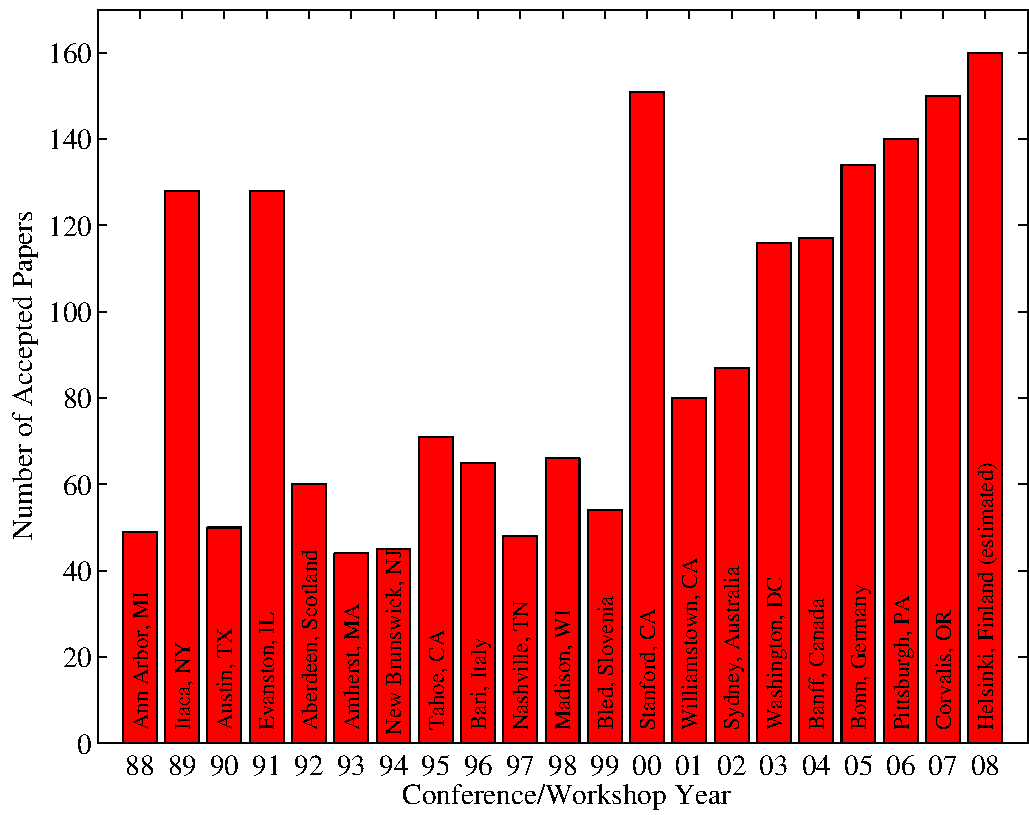
\includegraphics[width=\columnwidth]{icml_numpapers}}
\caption{Historical locations and number of accepted papers for International
Machine Learning Conferences (ICML 1993 -- ICML 2008) and International
Workshops on Machine Learning (ML 1988 -- ML 1992). At the time this figure was
produced, the number of accepted papers for ICML 2008 was unknown and instead
estimated.}
\label{icml-historical}
\end{center}
\vskip -0.2in
\end{figure}
\fi